\section{P-300 Prediction using Machine Learning}
Python programming language was used.\newline
The dataset II provided by competition III was in matlab files and ASCII. Due to being easier and more readable matlab files (*.mat) was used. There were 4 matlab files, 2 for each subject (A, B), 1 for training and the other for testing.

\subsection{Prepossessing}
Since the data is raw, certain preparations and calculations needs to be done in order to make it readable by the model. There exists 5 prepossessing calculations; 1 averaging of the repetitions and 4 filters to decrease and enhance the number of features.
\subsubsection{Averaging}
Each epoch consists of 12 intensifications and each intensification is repeated 15 times thus in order to decrease the noise, we take the average of each intensification for the 15 repetitions in 1 epoch.\newline
For easier future use, only Signal, StimulusCode and TargetChar arrays were used. For each epoch, a loop through StimulusCode array to search for a transition from non-zero to zero which means there was a transition from intensification to no intensification. Then, Taking the values of all channels from this index + start window - 24 to index + end window - 24. The index + start window - 24 because it takes the values of Signal from the start of the intensification with certain boost since we might not take the values from 0ms, as for index + end window - 24 to take the values of Signal for a whole second after the start of intensification given that end window = 240. Remember that 240 is the same as the digitization of the intercepted signal (240 samples = 1 second).
\subsubsection{Common Average Reference Filter}
Per epoch, Per intensification, we calculate the average of all 64 channels for a certain sample. then subtract each sample from the calculated average.\newline\newline
\begin{figure}
    \centering
    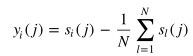
\includegraphics[width=70mm]{images/CAR-filter.jpg}
    \caption{Common Average Reference Equation}
    \label{fig:my_label}
\end{figure}
where s i(j) denotes the signal recorded on channel i at time j, y i(j) is the filtered signal after subtracting the mean of all channels and N is the number of channels [3].
\subsubsection{Moving Average Filter}
Per epoch, Per intensification, Per channel, the average of n consecutive samples is calculated and set the new signal values to the calculated average.
\subsubsection{Z-Score}
Per epoch, Per intensification, Per channel, Z-score is calculated.\newline\newline
\begin{figure}
    \centering
    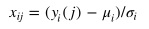
\includegraphics[width=70mm]{images/z-score.jpg}
    \caption{Z-Score Equation}
    \label{fig:my_label}
\end{figure}
where x ij denotes feature j of channel i (i.e. x i (j)), u i is the average of the signals recorded on channel i and o i is the
corresponding standard deviation.
\subsubsection{Decimation of Samples}
Finally, instead of taking all samples per channels, we take 1 per n consecutive samples, thus we decrease the number of features and keep the distinction of each feature as maximum as possible.
\subsubsection{Channel Concatenation}


\subsection{Model}
Only Least Discriminant Analysis (LDA) model was applied since it has the one of the highest scores for this dataset.\newline
The data segment consists of 800ms (start = 0, end = 192). and two sets of channels were used, the first one has the whole 64 channels, and the second has 8 channels (Fz, Cz, Pz, P3, P4, PO7, PO8 and Oz) as described in [2] in references.

\subsubsection{Plot of Wave Forms}
In order to signify the difference between the P300 wave form and non-P300 wave form, Figure 3.3 shows the P300 vs non-P300  for both subject A and B after taking the average of the chosen intensification for the entire 85 epochs.
\begin{figure}
    \centering
    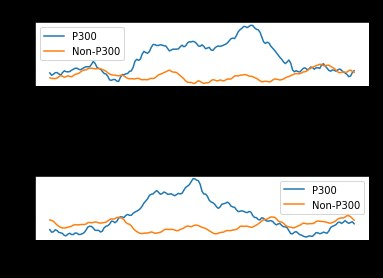
\includegraphics[width=70mm]{images/A-B-P300-plot.jpg}
    \caption{P300 for both subject A and B}
    \label{fig:my_label}
\end{figure}
\subsubsection{Least Discriminant Analysis}
Since the problem is a binary classification one, the line that signifies whether the signal is P300 or not can be calculated using the function in Figure 3.4.\newline
where x is the feature vector, w is the weight vector and b is the bias term [3]. \newline\newline
LDA is the easiest way to calculate this w using the equation in Figure 3.5.\newline
where x is the feature vector, y is class of each signal (1 for P300, -1 for non-P300).\newline\newline
In order to calculate which class the signal belongs to, the equation in Figure 3.6 is used.\newline
where x is the feature vector, w is the weight vector.\newline\newline
Since it is impossible to get 1 and -1 from the score function we take the max score within column and max score within rows to signify the chosen intersected character.
\begin{figure}
    \centering
    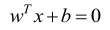
\includegraphics[width=70mm]{images/binary-classification-line-equation.jpg}
    \caption{Binary Classification Line Equation}
    \label{fig:my_label}
\end{figure}
\begin{figure}
    \centering
    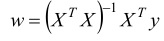
\includegraphics[width=70mm]{images/weight-calculation-lda.jpg}
    \caption{Weight Calculation Using LDA}
    \label{fig:my_label}
\end{figure}
\begin{figure}
    \centering
    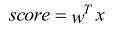
\includegraphics[width=70mm]{images/score-calculation-lda.jpg}
    \caption{Score Calculation Using LDA}
    \label{fig:my_label}
\end{figure}
\subsubsection{Results}
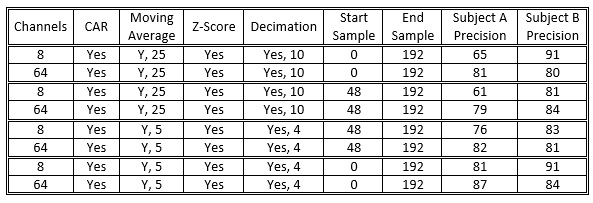
\includegraphics[width=70mm]{images/test-results.jpg}
